% Created 2023-05-13 Sat 19:52
% Intended LaTeX compiler: pdflatex
\documentclass[presentation]{beamer}
\usepackage[utf8]{inputenc}
\usepackage[T1]{fontenc}
\usepackage{graphicx}
\usepackage{longtable}
\usepackage{wrapfig}
\usepackage{rotating}
\usepackage[normalem]{ulem}
\usepackage{amsmath}
\usepackage{amssymb}
\usepackage{capt-of}
\usepackage{hyperref}
\usetheme{default}
\author{Miguel}
\date{\today}
\title{}
\hypersetup{
 pdfauthor={Miguel},
 pdftitle={},
 pdfkeywords={},
 pdfsubject={},
 pdfcreator={Emacs 27.1 (Org mode 9.4.6)}, 
 pdflang={English}}
\begin{document}

\begin{frame}{Outline}
\tableofcontents
\end{frame}

\begin{frame}[label={sec:orgc120f0f}]{Pokefetch}
\begin{block}{Dependencies}
\begin{itemize}
\item neofetch
\item jp2a
\item bash, shuf
\end{itemize}
\end{block}

\begin{block}{Neofetch Directory}
\begin{itemize}
\item Contains all pokemon sprites in separate folders.
\begin{itemize}
\item Pokemon:       contains all regular sprites
\item shiny:         contains the shiny ones
\item Unknown:       contains only Unknown
\item shiny\textsubscript{unknown}: contains the shiny Unknown
\end{itemize}
\end{itemize}
\end{block}
\end{frame}

\begin{frame}[label={sec:org5099c66},fragile]{Add to bashrc script Drop in}
 \begin{block}{All pokemon with 5\% shiny chance.}
\begin{verbatim}
# Remember to change ~/Path/to/neofetch below to make this work as expected
POKEFETCH_PATH=~/Path/to/neofetch
POKE=$( [ $(( RANDOM % (101) )) -gt 95 ] && echo $POKEFETCH_PATH/shiny/`ls $POKEFETCH_PATH/shiny|shuf -n 1` || echo    $POKEFETCH_PATH/Pokemon/`ls $POKEFETCH_PATH/Pokemon|shuf -n 1`)
neofetch --jp2a $POKE
\end{verbatim}
\end{block}

\begin{block}{Only the Unknown with 5\% shiny chance.}
\begin{verbatim}
# Remember to change ~/Path/to/neofetch below to make this work as expected
POKEFETCH_PATH=~/Path/to/neofetch
POKE=$( [ $(( RANDOM % (101) )) -gt 95 ] && echo $POKEFETCH_PATH/shiny_unknown/`ls $POKEFETCH_PATH/shiny_unknown|shuf -n 1` || echo    $POKEFETCH_PATH/Unknown/`ls $POKEFETCH_PATH/Unknown|shuf -n 1`)
neofetch --jp2a $POKE   --colors 10 12 0 12 15
\end{verbatim}
\end{block}
\end{frame}

\begin{frame}[label={sec:orgf64b45a},fragile]{Wrapper for neofetch}
 \begin{verbatim}
# This is to wrap the function of Pokefetch to work a little smoother. The ability to provide the main path to images as an argument.
# Assumes the user gives a directory that contains Pokemon/ as well as shiny/. Now you can curate your own selection to display instead of all of them. call like pokefetch /Path/to/pngs %d
# %d as percentage of normal
pokefetch()
{

POKEFETCH_PATH=$1
NORMAL=`ls $POKEFETCH_PATH/Pokemon|shuf -n 1`
SHINY=`ls $POKEFETCH_PATH/shiny|shuf -n 1`
   POKE=$( [ $(( RANDOM % (101) )) -gt $2 ] && echo $POKEFETCH_PATH/shiny/$SHINY || echo $POKEFETCH_PATH/Pokemon/$NORMAL)
   neofetch --jp2a $POKE --colors 10 12 0 12 15
   echo $NORMAL $SHINY


}
\end{verbatim}
\end{frame}


\begin{frame}[label={sec:orgd6ba79f}]{Examples}
\begin{figure}[htbp]
\centering
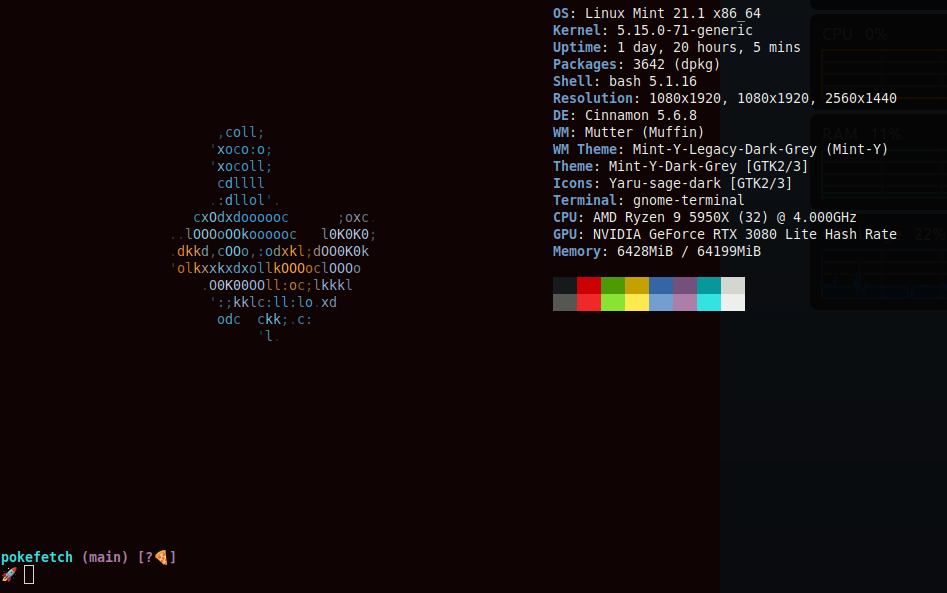
\includegraphics[width=.9\linewidth]{./images/Mudkip_example.png}
\caption{\label{fig:org80579d8}This is an example showing mudkip}
\end{figure}

\begin{figure}[htbp]
\centering
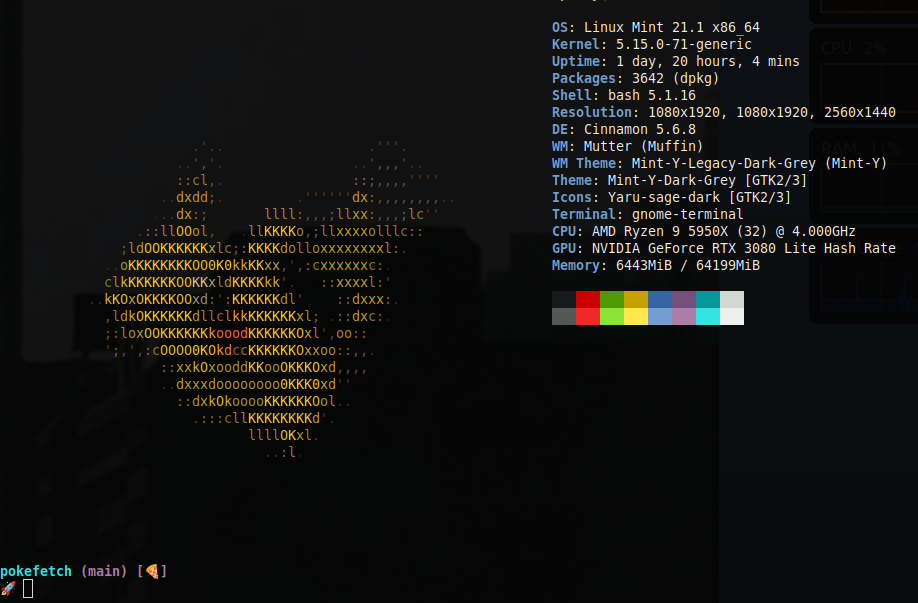
\includegraphics[width=.9\linewidth]{./images/Pikachu_example.png}
\caption{\label{fig:org4eb2b00}This is an example showing pikachu}
\end{figure}
\end{frame}
\end{document}